\chapter{Numerical Experiments}
\section{Constant Velocity}
\begin{figure}[H]
	\centering
	\begin{subfigure}[b]{0.5\textwidth}
		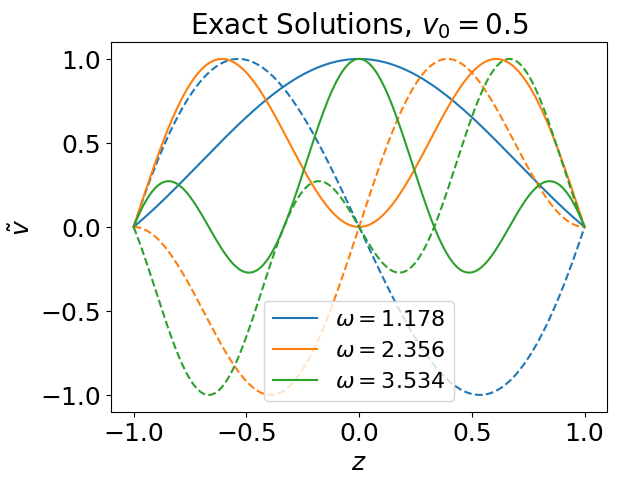
\includegraphics[width=\linewidth]{img/constant_v/exact-v0=0.5}
	\end{subfigure}%
	\begin{subfigure}[b]{0.5\textwidth}
		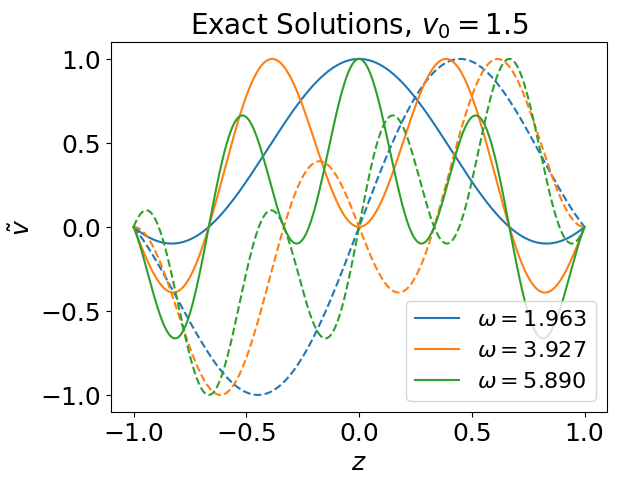
\includegraphics[width=\linewidth]{img/constant_v/exact-v0=1.5}
	\end{subfigure}
	\caption{Exact solution to the eigenvalue problem with constant velocity. The solid lines represent the real part of the eigenfunctions, and the dash lines represent the imaginary part.}
	\label{fig:exact}
\end{figure}

\subsection{Finite Difference}
\begin{figure}[H]
	\centering
	\begin{subfigure}[b]{0.5\textwidth}
		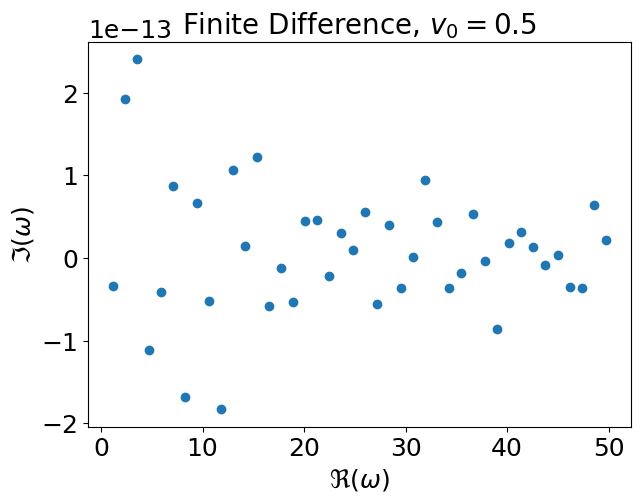
\includegraphics[width=\linewidth]{img/constant_v/eigenvals-fd-v0=0.5}
	\end{subfigure}%
	\begin{subfigure}[b]{0.5\textwidth}
		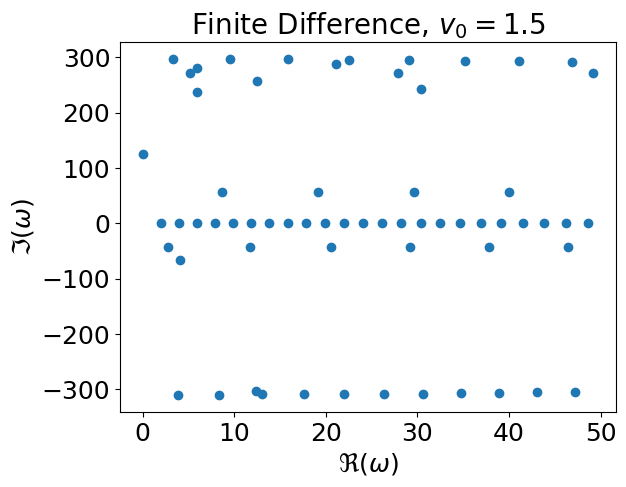
\includegraphics[width=\linewidth]{img/constant_v/eigenvals-fd-v0=1.5}
	\end{subfigure}
	\caption{The system is stable in subsonic case. However, spectral pollution occurs in the supersonic case, some spurious modes have imaginary frequency.}
	\label{fig:eigenvals-constant-v}
\end{figure}
\begin{figure}[H]
	\centering
	\begin{subfigure}[b]{0.5\textwidth}
		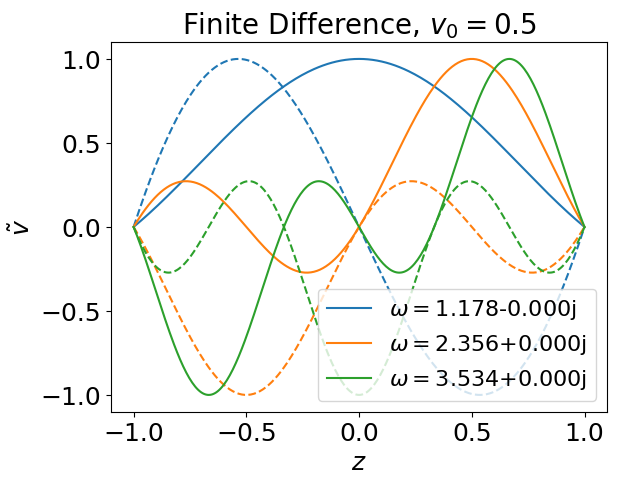
\includegraphics[width=\linewidth]{img/constant_v/eigenfuncs-fd-v0=0.5}
	\end{subfigure}%
	\begin{subfigure}[b]{0.5\textwidth}
		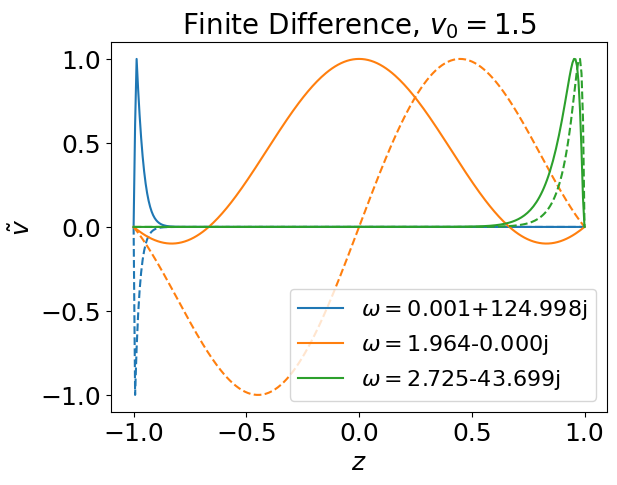
\includegraphics[width=\linewidth]{img/constant_v/eigenfuncs-fd-v0=1.5}
	\end{subfigure}
	\caption{For subsonic case, everything behaves good. However, spectral pollution occurs in the supersonic case, some spurious modes have imaginary frequency.}
	\label{fig:eigenfuncs-constant-v}
\end{figure}


\section{Subsonic Case}

\section{Supersonic Case}

\section{Transonic Case}